\documentclass[a4paper,12pt]{article}
\usepackage[utf8]{inputenc}
\usepackage{color,graphicx}
\usepackage[usenames,dvipsnames]{xcolor}
\graphicspath{{./}}
\usepackage{float} 

\usepackage{geometry}
 \geometry{
 a4paper,
 left=15mm,
 top=15mm,
 right=15mm, 
 bottom = 20mm,
 }

%opening
\title{Synaptic Imaging progress report}
\author{Tim Hanson, Filip Tomaska, Anthony Leonardo, jET team}

\begin{document}

\maketitle

\begin{abstract}

\end{abstract}

\section{Goals \& Motivation}

The goal of this project is to be able to measure synaptic weights -- that is, the effective coupling between pre- and post synapse -- in vivo, across a large number of synapses.  We also aim to measure the \textit{change} in synaptic weights as effected by learning or perception, on long and short time scales, respectively.  

Synapses are small, and labelling them is hard / yields few photons.  Based on these challenges, we have developed an Adaptive-Optics microscope, based around a MEMS deformable mirror, to optimize excitation and collection \textit{in vivo}.  To optically measure pre- and post-synaptic activity, you need multiple fluorescent indicators; to this end, the microscope is designed for dual-wavelength excitation and detection.  

We have primarily been experimenting with GluSnFR3 as a proxy for presynaptic activity (glutamate release) and jRGECO1a as a postsynaptic calcium indicator in cranial windowed mice.  Preliminary data from this and from experiments with far-red HaloCamp will be presented.  

\section{Optical system}

\subsection{Introduction}

Adaptive optics refers to the process of controlling the wavefront of light through an optical system.  Usually this is to correct for system or sample aberrations which cause light to decohere at focal planes.  Initial use of adaptive optics was for telescopes, where fast mirrors correct for wavefront errors induced by temperature-dependent refractive index changes in the atmosphere.  Later work by Betzing, Na Ji, and others showed that these same systems can be used to improve imaging with microscopes [].  

There are two different types of actuators used in adaptive optics microscopy: spatial light modulators (SLMs) and deformable mirrors (DMs).  SLMs have the advantage of many more degrees of freedom, as they are typically liquid-crystal on silicon (LCoS); the grayscale value written to the LC matrix directly modulates the wavefront phase.  Because of the high degrees of freedom, you can write phase gratings to SLMS and hence diffract light.  This permits pupil segmentation when optimizing a wavefront, a key advantage [].  

However, SLMs suffer from significant chromatic dependence: an AO optimization only works for the designed wavelength.  Given that we need to be multi-spectral to excite at least two different fluorescent indicators, this led us to go with a deformable mirror (DM). 

Deformable mirrors control the wavefront by flexing and moving a thin-membrane (usually coated silicon) mirror via electrostatic, electromagnetic, or piezoelectric actuators.  These mechanical devices can move quickly (milliseconds), but do have hysteresis, hence need to be controlled in a closed-loop manner through a wavefront sensor.  

There are two common ways of performing on-line correction of the wavefront: image-based methods and wavefront sensing\{footnote{There are other interferometric ways of measuring/correcting wavefront aberrations, but afaik these only work over small FOVs []}.  In image-based optimization, the wavefront (eg. excitation wavefront in a 2p scope, as here) is not directly measured, but is optimized based on the quality of the resultant image.  Pupil segmentation \& phase retrieval falls into this category [ref].  Wavefront sensing, in comparison, directly measures the wavefront, using a Shack-Hartmann sensor, of the emitted light, and can hence be used to correct aberrations.  

Because synapses are small, hard to label, fluorescent proteins are prone to bleaching, and the emitted light (green and red) is subject to scattering as well as index of refraction changes, we decided to use image-based wavefront adaptation.  In-vivo imaging of synapses is, in our hands, limited by photodamage and bleaching to the few-photons per pixel regime.  Wavefront sensing would not work well with such dim structures, even with advanced sensors like SPADs.  

\subsection{Detailed description}

Excitation light comes from a Coherent Discovery NX TPC, which provides a variable output (680 - 1320nm) and fixed output (1040nm).  Both outputs have built-in AOM power control, and the variable output has adjustable GDD compensation as well.  These two outputs are combined with a polarizing beam splitter, then expanded 3x with a Galilean beam expander.  

Scanning this beam is via a resonant-galvo-galvo system from a Thorlabs Bergamo II microscope, upon which the AO scope is directly built.  The 12kHz resonant X scanner and Y galvo are conjugated to prevent field walk-off in the pupil planes\footnote{Conjugated scan mirrors were originally specified as the original goal was to make a 2 photon STED microscope to maximize resolution.  STED, by design, reduces the total number of photons emitted, hence is best done with synthetic dyes designed to minimize bleaching under higher-state excitation and depletion.  Fluorescent protein based indicators would likely bleach too quickly under STED illumination.  We compromised on resolution to maximize signal, and use AO instead to improve resolution. },\footnote{The three scan lenses (two to conjugate and one 'actual' scan lens) were, per STED goals, originally specified for VIS-NIR transmission.  Given the demand for testing long-wavelength JF dyes, such as JF669 in the development of W-HaloCamp (Helen Farrants, Schreiter lab), we have replaced them with longer-wavelength NIR-MIR versions.}.  

The third scan lens forms a conjugate image plane (figure \ref{optical_schematic}).  A 685nm 50mW single-mode laser diode is imaged into this plane via a shortpass dichroic.  This light serves as an un-scanned reference beam for measuring the deformable mirror and performing closed-loop control.  Excitation and reference light then enter a tube lens, which forms a pupil plane on the deformable mirror.  Rather than using polarization optics \& another polarizing beam splitter, we illuminate the deformable mirror (22.5 mm pupil, 97 actuator, Alpao Inc.) at a 7.5deg incidence angle.  This leads to a degree of astigmatism, but modelling in Zemax showed this was tolerable due to the long working distance of the tube lenses.  This approach has the added benefit of folding the optical path, making it compatible with the Bergamo II footprint.  

The second tube lens leads to an intermediate image plane.  This is relayed and demagnified via a f=172 mm tube lens.  The demagnification makes the deformable mirror conjugate to the pupil plane of an Olympus 20x 1.0 NA objective (pupil diameter = 18 mm; DM image is 19.2mm, so objective is overfilled).  Prior the objective, wavefront sensor light is split from the excitation light via a second longpass dichroic mirror.  This is relayed onto a Shack-Harmann wavefront sensor (SHWFS) composed of a 14mm f.l. microlens array and 11 x 11mm CMOS sensor.  The relay demagnifies the objective pupil by 2.5x (f=100, AC254-100-B and two AC254-080-B), which increases the angular resolution of the SHWFS.  

This longpass dichroic also serves to separate epifluorescence excitation / emission light from the 2p excitation.  Epifluorescence imaging is essential for finding viral expression areas relative to surface vasculature (for example).  The actual epi arm is straightforward, and is presently fixed at GFP wavelengths (488 / 525 nm).  

Two-photon emitted light is detected via the red/green PMT arm.  This is taken, unmodified, from the original Bergamo II.  The PMTs work well for green/red emitted light, though there is some fixed-pattern noise, and are about half as sensitive at jf669 wavelengths (690nm).  As the second longpass dichroic is purposefully imperfect, some of the reference beam gets through the objective, hence a second longpass filter is inserted above the objective \& PMT arm to prevent contamination.  

When removed, this reference light has a second purpose: levelling the cranial window.  During experimentation we observed that significant sample aberrations come from angled cranial windows,  given the high NA of the objective.  To get a parallel beam of light out of the objective, we add a removable lens just before the custom tube lens to focus the reference beam at the pupil plane of the objective.  This results in collimated light to exit the objective, yielding a depth-insensitive back-reflected image off the window.  This light is split from the epifluorescence arm via a 650nm short-pass dichroic, and imaged onto a third camera via an lens f=175 mm lens.  The weak back-reflection from the cranial window is then compared to the stronger reflection off the surfaces of the objective, which by definition are on the optical axis, making it easy to adjust the angle of the headbar to make the window perpendicular.  

\begin{figure}
\label{optical_schematic}
\centering
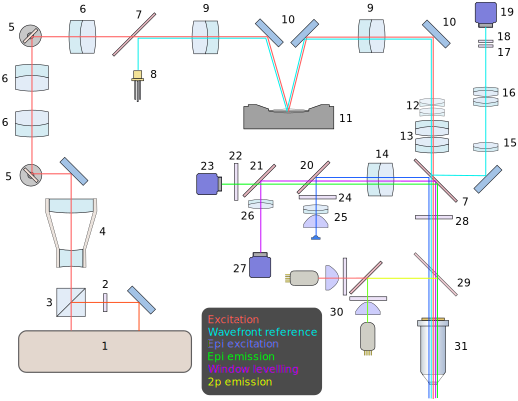
\includegraphics[width=\textwidth]{optical_schematic.pdf}
\caption{ Parts are from Thorlabs unless stated otherwise. 
\textbf{1} Dual output ultrafast laser, \textsl{Coherent Discovery NX TPC}. 
\textbf{2} Half Wave plate, \textsl{WPHSM05-1030}, on 1040 nm output. 
\textbf{3} Polarizing beam splitter, \textsl{PBS103}.
\textbf{4} 3x Beam expander, \textsl{GBE03-B}.
\textbf{5} 12kHz resonant Galvo mirror, \textsl{Cambridge Scientific}.
\textbf{6} f=50mm scan lens, \textsl{SL50-2P2}.
\textbf{7} Longpass dichroic mirror, 735 nm, \textsl{DMLP735B}.
\textbf{8} Laser diode, \textsl{HL6750MG}.
\textbf{9} f=200mm tube lens, \textsl{TL200-2P2}.
\textbf{10} 42mm x 60mm elliptic mirror, \textsl{Edmund Optics \#89-458}.
\textbf{11} Deformable mirror, \textsl{Alpao DM97-25}.
\textbf{12} Window levelling drop-in lens, \textsl{AC254-300-B} and \textsl{AC254-500-B}.
\textbf{13} Custom tube lens, \textsl{Edmund Optics \#49-386 and \#49-385}.
\textbf{14} Epi tube lens, \textsl{ TTL200-A}.
\textbf{15} Wavefront sensor pupil relay, \textsl{AC254-100-B}.
\textbf{16} Wavefront sensor pupil relay, \textsl{2x AC254-080-B}.
\textbf{17} Shortpass filter, \textsl{DMSP805}.
\textbf{18} Microlens array, f=14.6mm, 300um pitch,\textsl{MLA300-14AR}.
\textbf{19} CMOS Camera, \textsl{Basler acA2040-90um}.
\textbf{20} Longpass dichroic, 498 nm, \textsl{MD498}.
\textbf{21} Shortpass dichroic, 650nm, \textsl{DMSP650R}.
\textbf{22} Emission filter, \textsl{MF525-39}
\textbf{23} CMOS Camera, \textsl{ImagingSource DMK33UX249}.
\textbf{24} Excitation filter, \textsl{MF469-35}
\textbf{25} LED iluminator, \textsl{M450LP1}, aspheric condenser \textsl{ACL25416U}, f=75mm lens \textsl{LB1901-A}
\textbf{26} f=175mm lens, \textsl{LA4924-A}
\textbf{27} CMOS camera, \textsl{Basler acA2500-60um}
\textbf{28} Removable longpass, \textsl{Chroma ET780lp}
\textbf{29} Switchable longpass, from Bergamo II
\textbf{30} PMT arm from Bergamo II
\textbf{31} Objective, \textsl{Olympus XLUMPlanFL N 20x / 1.0 NA 2mm WD} 
}
\end{figure}

\begin{figure}
\label{CAD_layout}
\centering
\includegraphics[width=\textwidth]{CAD_layout.pdf}
\caption{CAD rendering of the microscope design, with salient parts labeled.  Left panel is view from the side, right panel view from the front, which shows the out-of plane epi excitation and levelling camera elements.  }
\end{figure}


As the initial window-leveling goniometer did not permit large range of motion about the cranial window, and windows over the mouse visual cortex tended to have significant angle, we designed a custom rotation stage for levelling the window, shown in figure \ref{window_level}.  This device is fabricated using waterjet cutting from 1/2`` stainless steel, and allows correction of up to $\pm 15^{\circ}$ in two directions. 

\begin{figure}
\label{window_level}
\centering
\includegraphics[width=4in]{window_levelling_CAD.png}
\caption{Window-levelling goniometer for rotating the mouse, headmount, and anesthesia system about the cranial window. }
\end{figure}

\subsection{Software control}

As mentioned above, the deformable mirror is nonlinear and has hysteresis, hence needs to be under closed-loop control of the SHWFS to function properly.  To perform closed-loop control, a custom C++ application acquires the wavefront image from the CMOS sensor of the SHWFS, process it to extract the centroid location, and compares these centroids to estimate the wavefront angle (derivative of the wavefront).  Based on the estimated wavefront angle and desired wavefront, the program adjusts drive current to the DM actuators.  

Dmitri Tsyboulski proved particularly helpful here, but the current control system differs from what he originally designed.  Normally, a wavefront sensor is calibrated with a known-flat measurement from a known source, such as an interferometer.  The interferometer was used extensively when testing centroid calculation, but in the actual system it's not used.  Instead, random actuator patterns are written to the DM while the resulting SHWFS centroid positions are recorded.  Many samples of the DM pattern -> SHWFS transform are recorded, typically 20k-200k.  These form an overspecified matrix mapping actuator setting (proportional to the slope of segments of the mirror) to $\Delta$ centroid position, relative to the \textsl{mean} centroid position.  In practice, these $\Delta$ centroid positions are $\pm 1-2$ pixels, so to improve SNR, centroid location is done via soft-threshold center-of-mass calculation, which results in centroid noise of $\sim$ 0.03 - 0.05 pixels (0.22$\mu m$ at the sensor, $< 0.01 \lambda $ wavefront resolution)).  The resultant system is fit with via least-squares regression so that: 

$$ (cp - mean(cp)) * M = a $$

Where $cp$ is the centroid position, $a$ are the actuator control values, and $M$ is the linear system control matrix.  Note that centroid position is two dimensional, so (x,y) pairs are concatenated to form the $cp$ vector on the left hand side of the expression above. $M$ is then used in a simple PI control loop to set the actuator values via $\delta cp * M = \delta a ; a = 0.995 * a - 0.5 \delta a$ -- you set the wavefront by controlling the 'mean' wavefront or roughy what the system considers to be 'flat'.  This is somewhat slow, needing ~100ms to settle (5 frames; wavefront sensor runs at 50 fps) , but given that so far we haven't needed to change wavefront quickly, no efforts have been made to further accelerate it.  

The software also allows the ability to control wavefront modally, using Zernike coefficients.   To this end, a Matlab script calculates the x and y derivatives of the Zernike poynomials at the (normalized) centroid positions.  Then 'flat' in the PV controller is simply the per-mode weighted sum of each of these derivatives plus calibrated system 'flat'.  This is used when doing modal AO correction.  

We have also experimented with controlling the wavefront modally based on the singular value dimensions of the optimization matrix.  The motivation for this is that if the black-box optimizer (next section) moved primarily in a subspace of the full 97-dimensions permitted by the DM when improving image quality on a sample, then it may benefit to optimize along these dimensions \textit{in vivo} as well.  This turned out not to be the case!  

[insert a figure of the software] 

\subsection {AO optimization}

Having no true calibrated flat, we needed some way of measuring and compensating for system aberrations, including those caused by imperfections in the DM.  To do this, we repeatedly image polystyrene fluorescent beads embedded in coverslip sealant while continually varying the DM command signal.  By then measuring the brightness of the image (proportional to the squared intensity of the excitation light, hence sensitive to PSF size), we can run closed-loop black-box optimization over the DM control signal while recording the resulting SHWFS signal.  A genetic algorithm is used for optimization, with Gaussian scalar mutation driven by a global, linearly-decreasing temperature, 20\% chance of overall mutation, and topology-aware recombination that occurs by dividing the DM actuators into 'mom' and 'dad' by an arbitrary chord through the center.  This genetic algorithm is able to reliably retrieve 'nearly optimal' wavefront setting after 15k samples from the DM settings (which is a very small proportion of the fully 97-dimensional space).  Note that we do not control or record the DM settings directly, but rather the resulting SHWFS centroid positions.  Optimal settings then serve as a 'reference flat' (as described above) that can be switched dynamically based on the wavelength required.  

While quantum dots bleach slowly, they do bleach, making it essential to dynamically de-trend the fluoresence during optimization, and then de-trend the best 100 wavefronts before solving for the 'flat'.

\begin{figure}
\centering
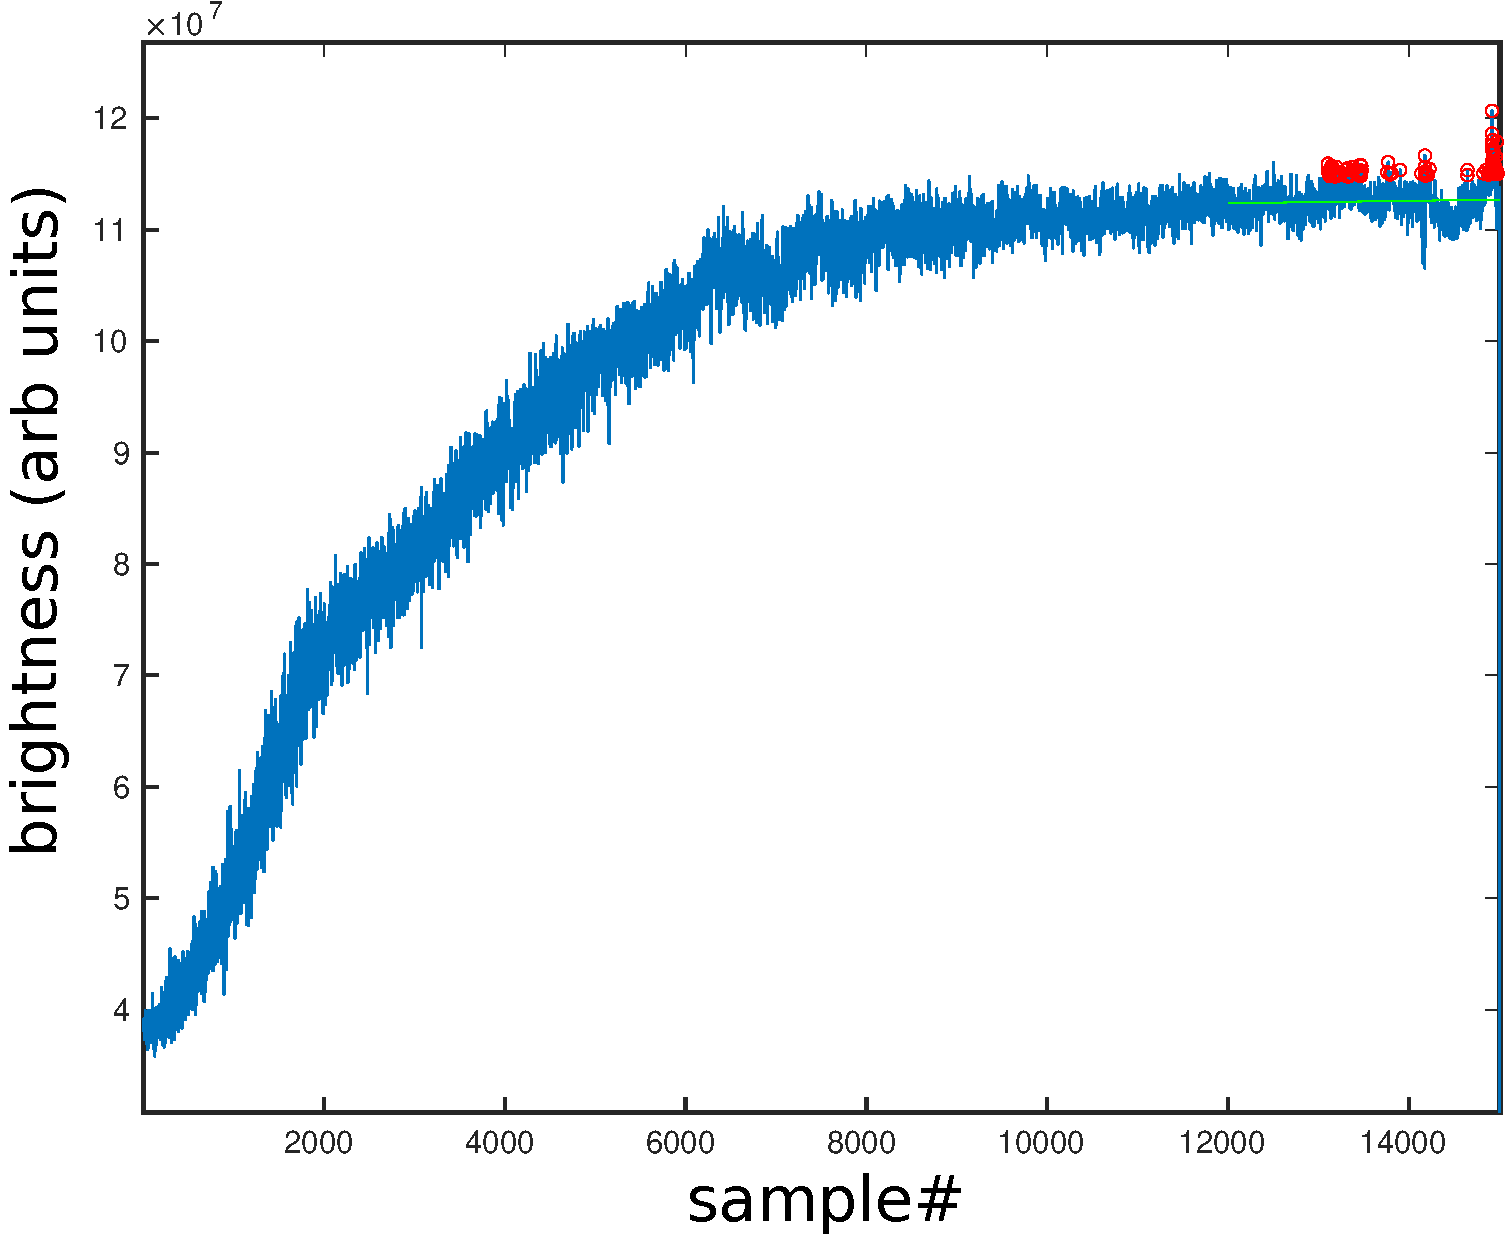
\includegraphics[width=4in]{PSbeads_optimization_run.pdf}
\caption{Example run showing $\sim$3x improvement in brightness from naive flat (no command signal written to the DM).  This was done with PS beads embedded in coverslip sealant; due to the lower partial pressure of oxygen in this matrix, bleaching was almost absent, and this serves as the best calibration to date.}
\end{figure}

\section{Experimental testing}

\subsection{Preliminary testing in slices}

At the beginning of the pandemic, we tested and validated the system in acute mouse brain slices.  This, unsurprisingly, is a challenging task; I never did get calcium transients, but was able to validate imaging two-color imaging of morphology. Chris Magnus was particularly helpful with guidance on making and maintaining slices. 

Two-color imaging is not, of course, particularly challenging (most 2p microscopes include dual PMTs, red and green), but to ascertain that the fixed 1040 nm output of the Chameleon would work we stained wildtype mouse coronal brain slices with SynaptoGreen and SynaptoRed dye.  Both are water-soluble but moderately lipophillic dyes that localize, to a varying extent, to vacuoles and synaptic vesicles; we observed decent contrast between white matter and cells, see figure \ref{synapto_green_red}. 


\subsection{GluSnFR3}

Link to movies here / do some sort of analysis of spine variance based on movies we have. 

\subsection{W-Halocamp}

Initial results here too!  Enough change in fluorescence to measure.  

\subsection{jRGECO1a x GluSnFR3}

Very preliminary results here.  Yet it does seem to be working. 

\section{Conclusions}

\end{document}
